\documentclass{article}

\usepackage{amsmath}
\usepackage{amsfonts}
\usepackage{amssymb}
\usepackage{amsthm}
\usepackage{graphicx}
\usepackage{subcaption}
\usepackage{siunitx}
\usepackage[margin=0.5in]{geometry}

\title{Homework 4}
\author{Miguel Angel Gomez Barrera}

\begin{document}
	\maketitle
\paragraph{1.} Implement the "Super random" number generator in python.
\paragraph{} The code of the generator is on the file "\textit{RunMeInPython.py}".
\paragraph{2.} We learned in class about Monte Carlo Integration and in particular computed the following:
$$I = \int_{0}^{1} e^{-x^2} \approx 0.7468241328.$$
\paragraph{}Plot the function in that interval and using the Monte Carlo method described in class, compute that integral for $N = 10000$. What value do you get? What is the error? How do you compute it?
\begin{figure}[h!]
	\centering
	\begin{subfigure}[b]{0.5\linewidth}
		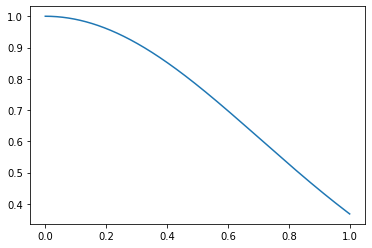
\includegraphics[width=\linewidth]{fn.png}
		\caption{The function.}
	\end{subfigure}
	\newline
	\begin{subfigure}[b]{0.45\linewidth}
		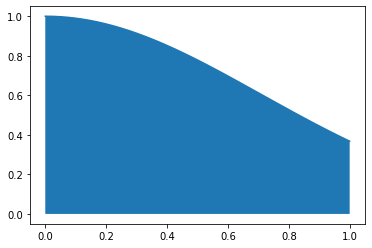
\includegraphics[width=\linewidth]{fn_area.png}
		\caption{The integral of the function: $\approx 0.7468241328$.}
	\end{subfigure}
	\begin{subfigure}[b]{0.45\linewidth}
		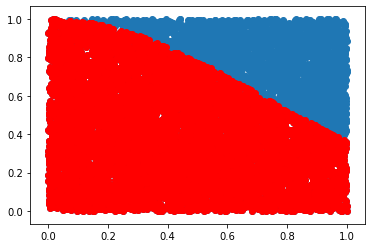
\includegraphics[width=\linewidth]{fn_monte_carlo.png}
		\caption{Monte Carlo approximation of the integral: $\approx 0.7468$.}
	\end{subfigure}
\end{figure}
\paragraph{} The Monte Carlo approximation is really close to the expected value, but to be honest this is only because of the way the collection of numbers was chosen by the computer algorithm, other results are: $0.7465, 0.7502, 0.7475, \dots$, then we can compute the error as the difference between the expected value and the approximation: \num{2.41328e-5}, \num{3.41328e-4}, \num{-3.3758672e-3} and \num{-6.758672e-4}. But not in all cases an expected value will be given, then, how we can compute the error? we can be sure by the method itself, that depends on two factors: The first one, is determined by the number of points we choose to include in our interval (the N parameter), in this computation we used $N=10000$, but if we choose $N=1000,100, 10$ or $1$ we would have a greater error, by his argument, we can state that an increase in $N$ gives us a better approximation; second, the random number generator should be 'random', the argument here lies in the numbers generated, they should be uniform in the interval that we are interested.
\begin{center}
	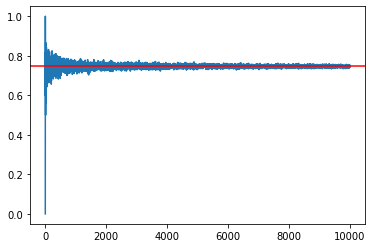
\includegraphics[width=0.7\linewidth]{error_convergence.png}
\end{center}
\paragraph{} This graph represents N versus the approximate value, we see that as N increases the approximation tends to the real value, if we look closely between $9000$ and $10000$ see the same effect.
\begin{center}
	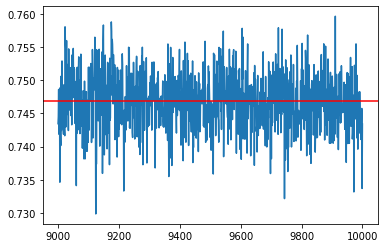
\includegraphics[width=0.7\linewidth]{error_convergence_closer.png}
\end{center}
\paragraph{}The points tend to be around a central value (our target value), then an statistical measure such as deviation (of the means), could be used to estimate the error.
\begin{equation}
	M = \frac{\sum_{n=1}^{i}S_n}{i} 
\end{equation}
\begin{equation}
	E = \sqrt{\frac{\sum_{n=1}^{i} (S_n - M)^2}{i}}	
\end{equation}
Where $M$ is the mean of the values and $E$ the error function and $i$ is the number of samples. Using this equations on the montecarlo simulation data from $1$ to $10000$ we get:
\begin{figure}[h!]
	\centering
	\begin{subfigure}[b]{0.45\linewidth}
		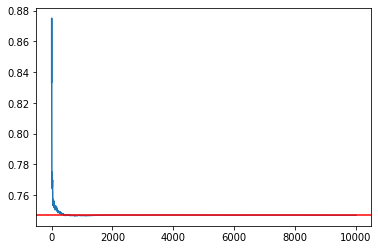
\includegraphics[width=\linewidth]{means_vs_real.png}
		\caption{The mean of the estimates vs the real value.}
	\end{subfigure}
	\begin{subfigure}[b]{0.45\linewidth}
		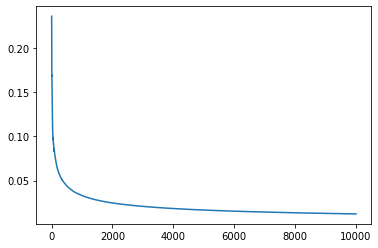
\includegraphics[width=\linewidth]{error_fn.png}
		\caption{The error function as we increase $N$.}
	\end{subfigure}
\end{figure}
\paragraph{} Notice that we did not use the actual value to compute the error function. By the central limit theorem these values will be normally distributed around a mean (in this case the value that we want to approximate).
\paragraph{} The code files to compute these graphs are:
\begin{itemize}
	\item \textit{montecarlo\_integration.py}.
	\item \textit{multi\_plot.py}.
	\item \textit{multi\_plot\_error.py}
\end{itemize}
\end{document}